
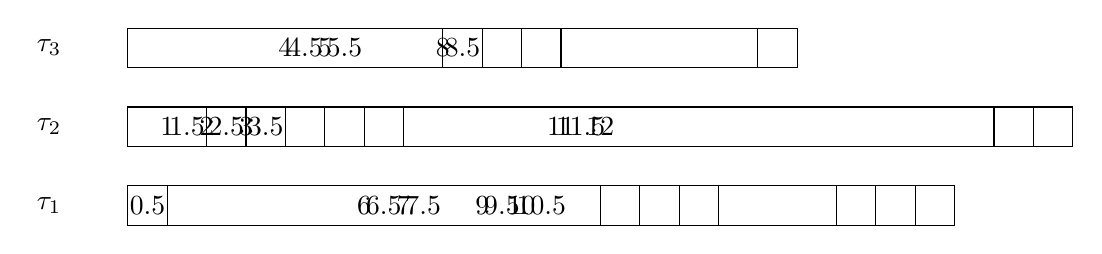
\begin{tikzpicture}
\node at(-1, 0.25) {$\tau_1$};
\node at(-1, 1.25) {$\tau_2$};
\node at(-1, 2.25) {$\tau_3$};
\draw[draw=black] (0, 0) rectangle ++(0.5,0.5) 
       node[pos=.5] {0.5};
\draw[draw=black] (0, 1) rectangle ++(1,0.5) 
       node[pos=.5] {1};
\draw[draw=black] (0, 1) rectangle ++(1.5,0.5) 
       node[pos=.5] {1.5};
\draw[draw=black] (0, 1) rectangle ++(2,0.5) 
       node[pos=.5] {2};
\draw[draw=black] (0, 1) rectangle ++(2.5,0.5) 
       node[pos=.5] {2.5};
\draw[draw=black] (0, 1) rectangle ++(3,0.5) 
       node[pos=.5] {3};
\draw[draw=black] (0, 1) rectangle ++(3.5,0.5) 
       node[pos=.5] {3.5};
\draw[draw=black] (0, 2) rectangle ++(4,0.5) 
       node[pos=.5] {4};
\draw[draw=black] (0, 2) rectangle ++(4.5,0.5) 
       node[pos=.5] {4.5};
\draw[draw=black] (0, 2) rectangle ++(5,0.5) 
       node[pos=.5] {5};
\draw[draw=black] (0, 2) rectangle ++(5.5,0.5) 
       node[pos=.5] {5.5};
\draw[draw=black] (0, 0) rectangle ++(6,0.5) 
       node[pos=.5] {6};
\draw[draw=black] (0, 0) rectangle ++(6.5,0.5) 
       node[pos=.5] {6.5};
\draw[draw=black] (0, 0) rectangle ++(7,0.5) 
       node[pos=.5] {7};
\draw[draw=black] (0, 0) rectangle ++(7.5,0.5) 
       node[pos=.5] {7.5};
\draw[draw=black] (0, 2) rectangle ++(8,0.5) 
       node[pos=.5] {8};
\draw[draw=black] (0, 2) rectangle ++(8.5,0.5) 
       node[pos=.5] {8.5};
\draw[draw=black] (0, 0) rectangle ++(9,0.5) 
       node[pos=.5] {9};
\draw[draw=black] (0, 0) rectangle ++(9.5,0.5) 
       node[pos=.5] {9.5};
\draw[draw=black] (0, 0) rectangle ++(10,0.5) 
       node[pos=.5] {10};
\draw[draw=black] (0, 0) rectangle ++(10.5,0.5) 
       node[pos=.5] {10.5};
\draw[draw=black] (0, 1) rectangle ++(11,0.5) 
       node[pos=.5] {11};
\draw[draw=black] (0, 1) rectangle ++(11.5,0.5) 
       node[pos=.5] {11.5};
\draw[draw=black] (0, 1) rectangle ++(12,0.5) 
       node[pos=.5] {12};
\end{tikzpicture}
